\label{sec:configuration}
This section is intended to provide guidelines for RTA-SUM DIAG configuration. 

\section{Configuration Parameters}
RTA-SUM DIAG parameters are divided in two containers: DiagGeneral (Figure \ref{fig:general_container}) and DiagConfigSet (Figure \ref{fig:configSet_container_0}).

\subsection{DiagGeneral}
\label{subsection:general}
This container comprises the general parameters of the module.

\begin{figure}[H]
	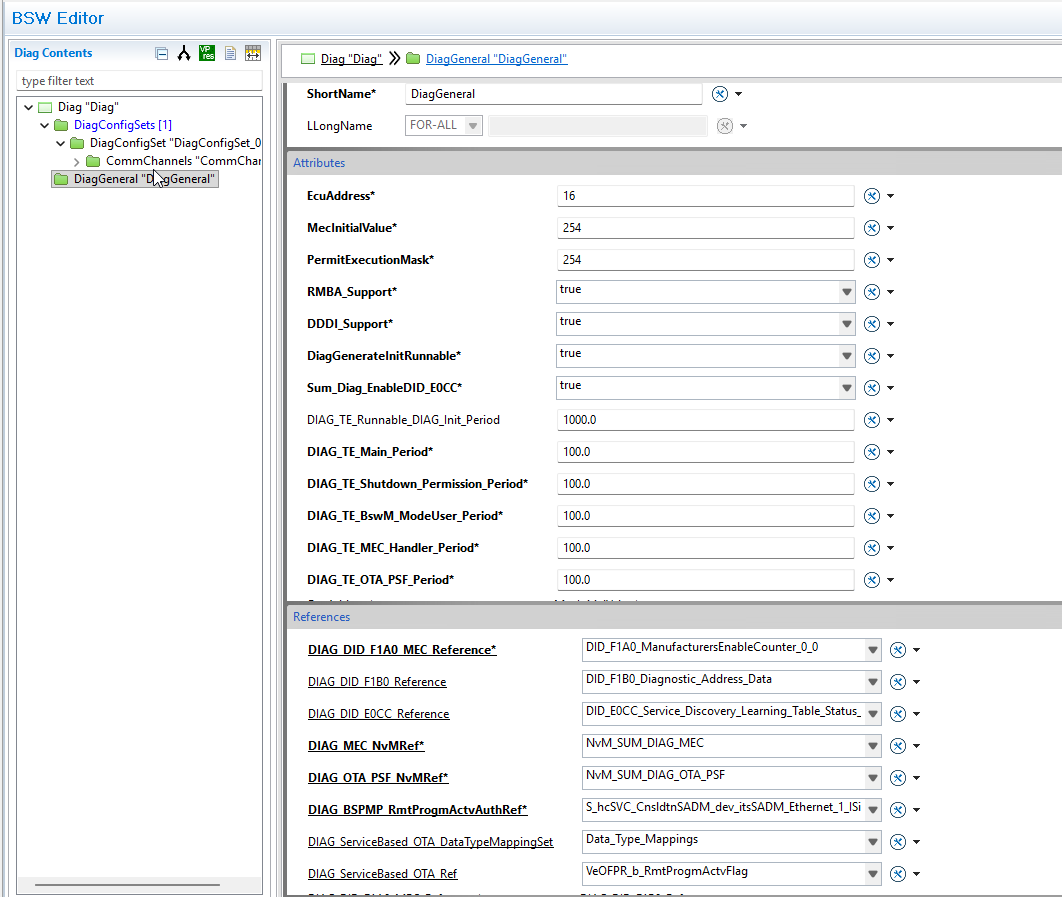
\includegraphics[width=1\textwidth]{images/General.png}
	\caption{RTA-SUM DIAG General Container.}
	\label{fig:general_container}
\end{figure} 

\textbf{EcuAddress:} ECU address.

\textbf{MecInitialValue:} Manufacturer Enable Counter (MEC) Initial Value.

\textbf{PermitExecutionMask:} PermitExecution mask to start execution of RTA-SUM DIAG module.

\textbf{RMBA\_Support:} RMBA\_Support is used to check if ECU supports Read Memory by Address service of DCM.

\textbf{DDDI\_Support:} DDDI\_Support is used to check if ECU supports Dynamically Define Data By Memory Address service.

\textbf{DiagGenerateInitRunnable:} DiagGenerateInitRunnable is used to generate a periodic runnable entity to call DIAG initiation function only once.

\textbf{Sum\_Diag\_EnableDID\_E0CC:} Sum\_Diag\_EnableDID\_E0CC is used to enable/disable support for DID 0xE0CC (Service Discovery Learning Table Status). When enabled, interfaces and code for DID E0CC are generated. When disabled, SrvcMgr provides an alternative implementation.

\textbf{DIAG\_TE\_Runnable\_DIAG\_Init\_Period:} DIAG\_TE\_Runnable\_DIAG\_Init\_Period is used to specify the periodicity, in milliseconds, of the initialization runnable.

\textbf{DIAG\_TE\_Main\_Period:} DIAG\_TE\_Main\_Period is used to specify the periodicity, in milliseconds, of the Main runnable.

\textbf{DIAG\_TE\_Shutdown\_Permission\_Period:} DIAG\_TE\_Shutdown\_Permission\_Period is used to specify the periodicity, in milliseconds, of the Shutdown Permission runnable.

\textbf{DIAG\_TE\_BswM\_ModeUser\_Period:} DIAG\_TE\_BswM\_ModeUser\_Period is used to specify the periodicity, in milliseconds, of the BswM Mode runnable.

\textbf{DIAG\_TE\_MEC\_Handler\_Period:} DIAG\_TE\_MEC\_Handler\_Period is used to specify the periodicity, in milliseconds, of the MEC handler runnable.

\textbf{DIAG\_TE\_OTA\_PSF\_Period:} DIAG\_TE\_OTA\_PSF\_Period is used to specify the periodicity, in milliseconds, of the OTA PSF runnable.

\textbf{DIAG\_ServiceBased\_OTA\_DataTypeMappingSet:} Foreign reference to the DATA-TYPE-MAPPING-SET in the system extract used for OTA service-based operations. This parameter references the system data type mapping set that defines the structure and format for OTA service-based functionality and data transformations.

\textbf{DIAG\_MEC\_NvMRef:} DIAG\_MEC\_NvMRef is used to refer to the NvM MEC NvMBlockDescriptor. 

\textbf{DIAG\_OTA\_PSF\_NvMRef:} DIAG\_OTA\_PSF\_NvMRef is used to refer to the NvM OTA PSF NvMBlockDescriptor.

\textbf{DIAG\_BSPMP\_RmtProgmActvAuthRef:} Reference to the Backup System Power Mode Protected: Remote Programming Active Authenticated signal.

\textbf{DIAG\_DID\_F1A0\_MEC\_Reference:} Reference to the Dcm Data for DID F1A0.

\textbf{DIAG\_DID\_F1B0\_Reference:} Reference to the Dcm Data for DID F1B0.

\textbf{DIAG\_DID\_E0CC\_Reference:} Reference to DCM DID E0CC (Service Discovery Learning Table Status) data.

\textbf{DIAG\_ServiceBased\_OTA\_Ref:} Foreign reference to the IMPLEMENTATION-DATA-TYPE-ELEMENT for Service Based OTA operations from the System Extract. This reference points to the specific implementation data type element used for OTA service-based functionality within the software architecture packages.

\subsection{DiagConfigSet}
This container comprises the communication channels configuration.

\begin{figure}[H]
	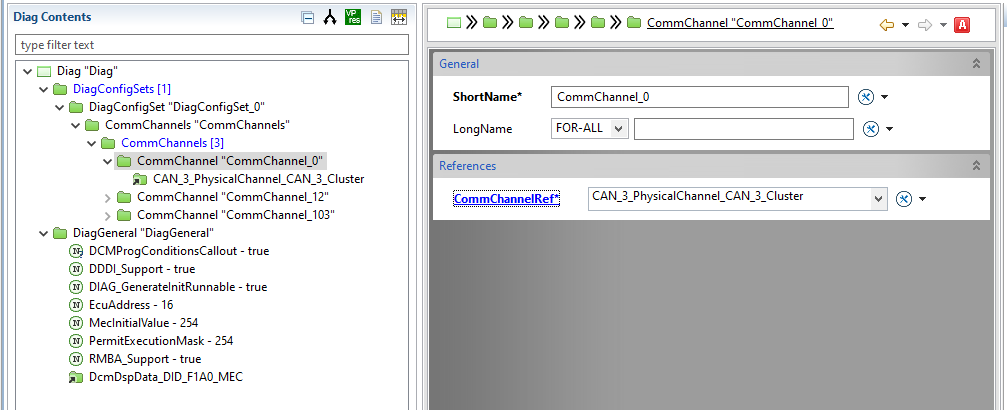
\includegraphics[width=1\textwidth]{images/CommChannel_Config_Step0.png}
	\caption{RTA-SUM DIAG ConfigSet Container.}
	\label{fig:configSet_container_0}
\end{figure} 

\textbf{CommChannelRef: } Reference to the Com Channel in the ComM module.

\section{Configuration Hints}
\subsection{Mandatory Parameter Validation}
\label{sec:inputvalidation}
RTA-SUM DIAG performs input validation on the ARXML BAMF configuration parameters.
If a mandatory parameter is not configured, RTA-CAR will stop the code generation and report an error identifying the missing or invalid parameter.

Ensure all mandatory parameters are properly set before executing the code generation. The following behavior applies:

\begin{itemize}
	\item If a mandatory parameter is missing or left unconfigured, RTA-CAR halts the generation and outputs an error message specifying the affected parameter.
	\item The generation will not proceed until all mandatory parameters are correctly provided.
	\item Review the reported error to identify and resolve any missing or invalid parameter configuration.
\end{itemize}

\begin{figure}[H]
	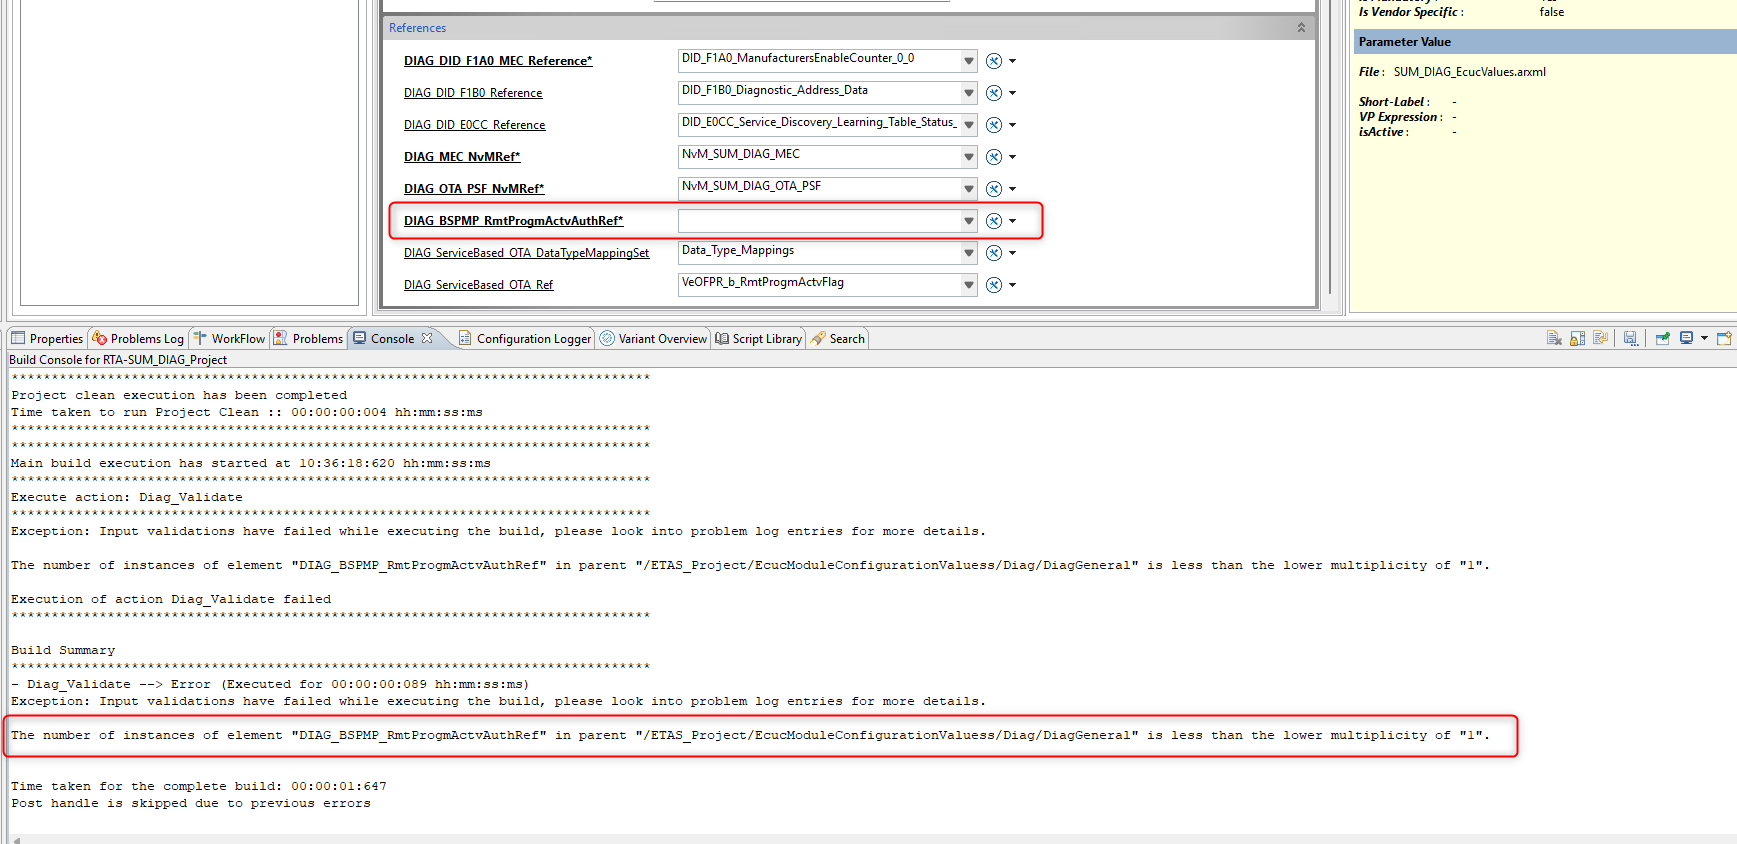
\includegraphics[width=1\textwidth]{images/MandatoryParamMissing.png}
	\caption{RTA-CAR error example for missing mandatory parameter.}
	\label{fig:MandatoryParamMissing}
\end{figure}

\subsection{MEC Interfaces}
Contains PPort Connections used by SUM\_DIAG to communicate to other modules to MEC value.

\begin{itemize}
	\item \code{PP_DIAG_SOH_GetMEC} connects with RPort of \code{SUM_SOH}.
	\item \code{PP_DIAG_SSC_GetMEC} connects with RPort of \code{SUM_SSC}.
	\item \code{PP_DIAG_SSFM_GetMEC} connects with RPort of \code{SUM_SSFM}.
\end{itemize}

\subsection{OTA-PSF Flag}
\label{sec:otaflag}
SUM\_DIAG needs to retrieve, calculate and provide the current OTA-PSF flag. 
To do that, it needs to read the value of \textit{RmtProgmActvAuth} of the Backup System Power Mode Protected message.
This value is provided by the Com module via the BSPMP\_RmtProgmActvAuth\_Signal port interface and forwarded to the SUM\_SSFM and Swcs via the DIAG\_RmtPrgmOtaPsf port interface.
For this purpose, the signal must be referenced in the DIAG\_BSPMP\_RmtProgmActvAuthRef.

\begin{figure}[H]
	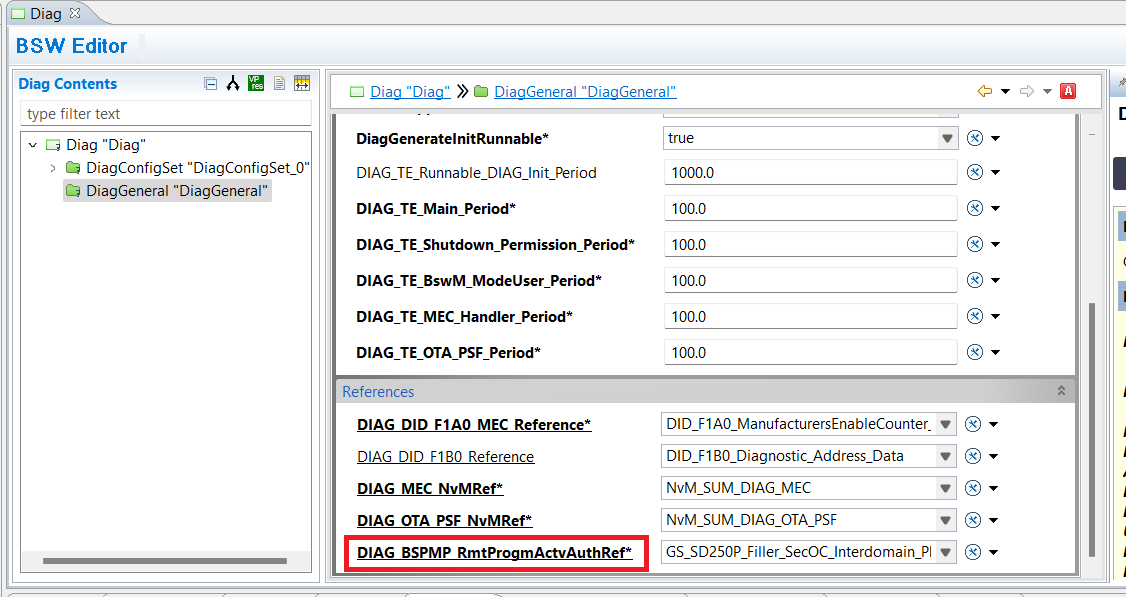
\includegraphics[width=1\textwidth]{images/RmtProgmActvAuthRef.png}
	\caption{ RTA-SUM DIAG network signal reference}
	\label{fig:RmtProgmActvAuthRef}
\end{figure}

\subsubsection{Service-Based OTA Configuration}
\label{sec:servicebasedota}
For service-based OTA operations, SUM\_DIAG requires additional configuration to properly reference the system data type mappings and implementation data type elements. Two new parameters enable this functionality:

\textbf{DIAG\_ServiceBased\_OTA\_DataTypeMappingSet Configuration:}
This foreign reference parameter configures the reference to the DATA-TYPE-MAPPING-SET in the system extract. The parameter must be configured to point to the correct data type mapping set used for OTA service-based operations.

\textbf{DIAG\_ServiceBased\_OTA\_Ref Configuration:}
This foreign reference must be configured to point to the specific IMPLEMENTATION-DATA-TYPE-ELEMENT that contains the OTA service-based functionality within the software architecture packages. This reference establishes the connection between the diagnostic module and the system's OTA implementation data types.

\begin{figure}[H]
	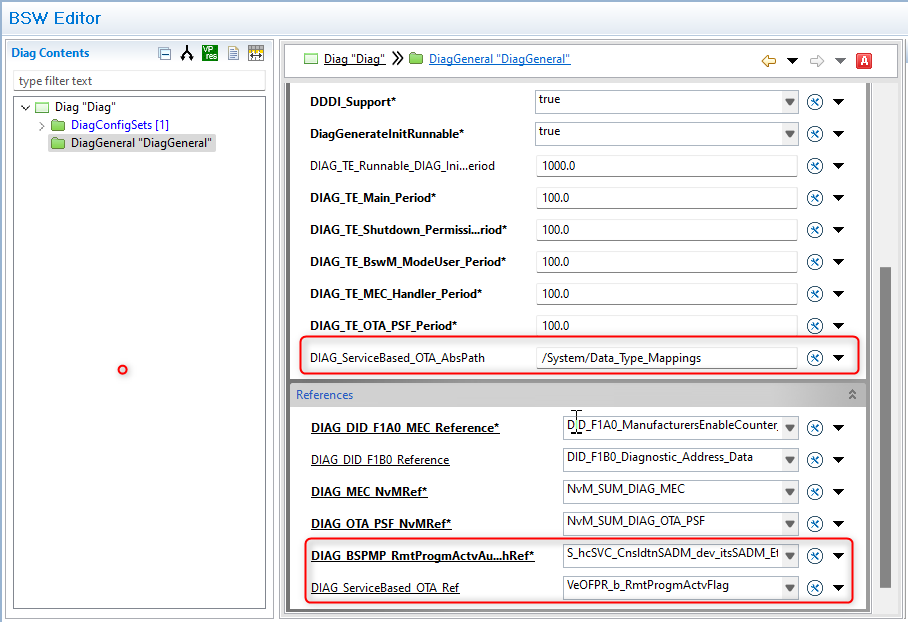
\includegraphics[width=1\textwidth]{images/servicebasedota.png}
	\caption{ RTA-SUM DIAG Service-Based OTA}
\end{figure}

\textbf{Configuration Dependencies:}
When configuring service-based OTA operations, ensure that:
\begin{itemize}
	\item The \texttt{DIAG\_ServiceBased\_OTA\_DataTypeMappingSet} references a valid DATA-TYPE-MAPPING-SET in the system extract
	\item The \texttt{DIAG\_ServiceBased\_OTA\_Ref} references an existing IMPLEMENTATION-DATA-TYPE-ELEMENT
	\item The referenced implementation data type element is properly defined in the system architecture
	\item The data type mappings are consistent with the system's OTA service implementation
\end{itemize}

\subsection{ControlDTCSetting}
\label{sec:controldtc}
The SUM\_DIAG module needs a BswM Mode Switch interface to receive the result of the Control DTC setting changes and
uses this information in the preconditions of the UDS Indications and Confirmations.

\subsubsection{DCM Configuration}
For this purpose, the user shall firstly enable the \textbf{DcmSupportDTCSettingControlOptionRecord}  parameter in the DCM module.

\begin{figure}[H]
	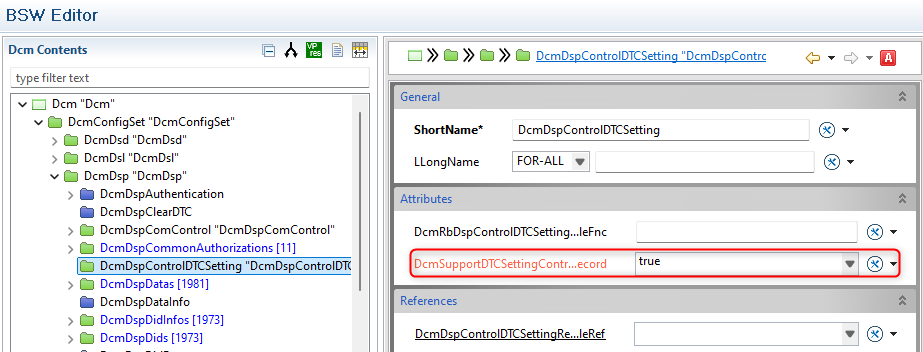
\includegraphics[width=1\textwidth]{images/DcmSupportDTCSettingControlOptionRecord.png}
	\caption{RTA-BSW DCM DcmSupportDTCSettingControlOptionRecord}
	\label{fig:configSet_DcmSupportDTCSettingControlOptionRecord}
\end{figure} 

By executing the BSW generation, the DCM will create a new port interface \textbf{DcmControlDTCSetting} (Figure \ref{fig:Pp_DcmControlDTCSetting})
and a Mode Declaration group \textbf{MDGP\_DcmControlDTCSetting} that will be the inputs for the BswM module.

\begin{figure}[H]
	\includegraphics[width=1\textwidth]{images/Pp\_DcmControlDTCSetting.png}
	\caption{DcmControlDTCSetting}
	\label{fig:Pp_DcmControlDTCSetting}
\end{figure} 


\subsubsection{BswM Configuration}
Now we need to use those generated items in the BswM. 

Firstly, we need to create a \textit{BswMModeRequestPort} (Figure \ref{fig:BswMModeRequestPort}) with a sub-container of type \textit{BswMSwcModeNotification} that references the 
MDGP\_DcmControlDTCSetting of the DCM.

\begin{figure}[H]
	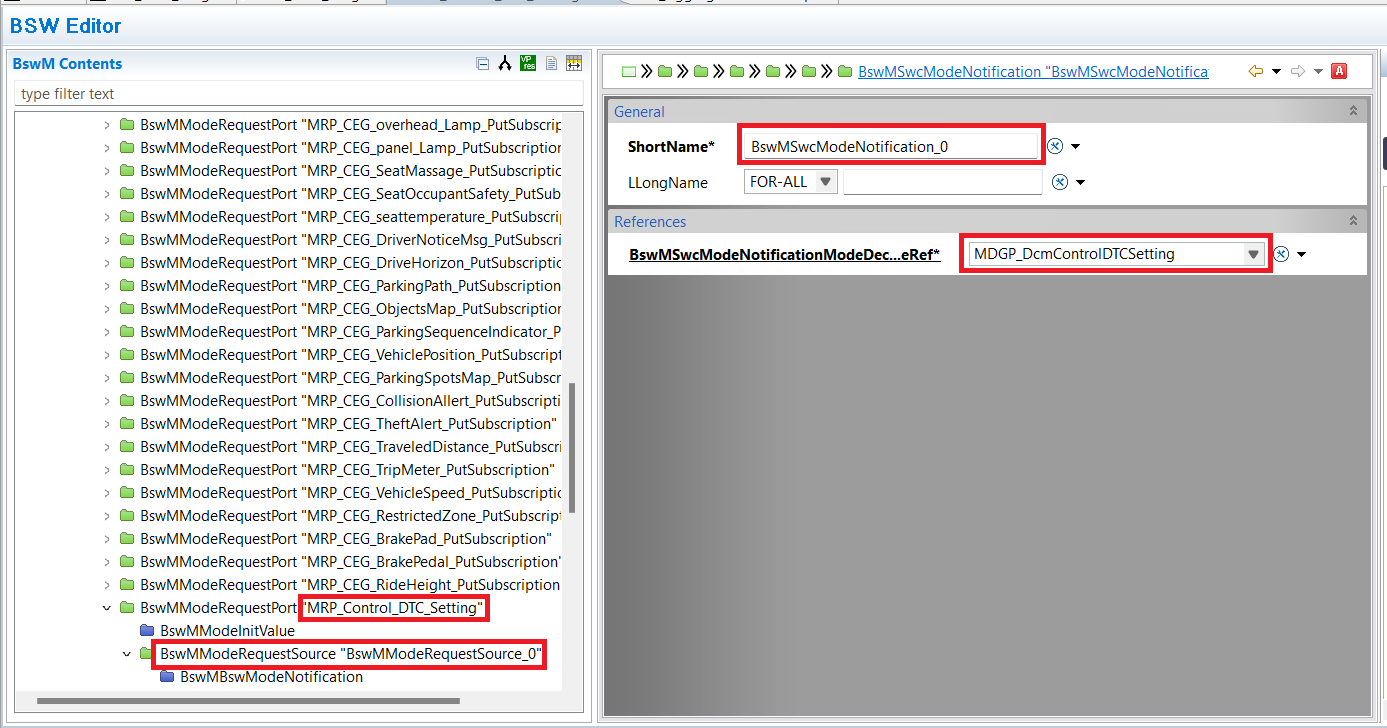
\includegraphics[width=1\textwidth]{images/BswM0.png}
	\caption{RTA-BSW BswM BswMModeRequestPort}
	\label{fig:BswMModeRequestPort}
\end{figure} 

Now, it is necessary to create the two \textit{Conditions} (Figure \ref{fig:Conditions}) for ENABLED and DISABLED states of the DTC setting control. 

Use the /AUTOSAR\_Dcm/ModeDeclarationGroups/DcmControlDTCSetting in the condition reference.

Here an example of configuration:

\begin{figure}[H]
	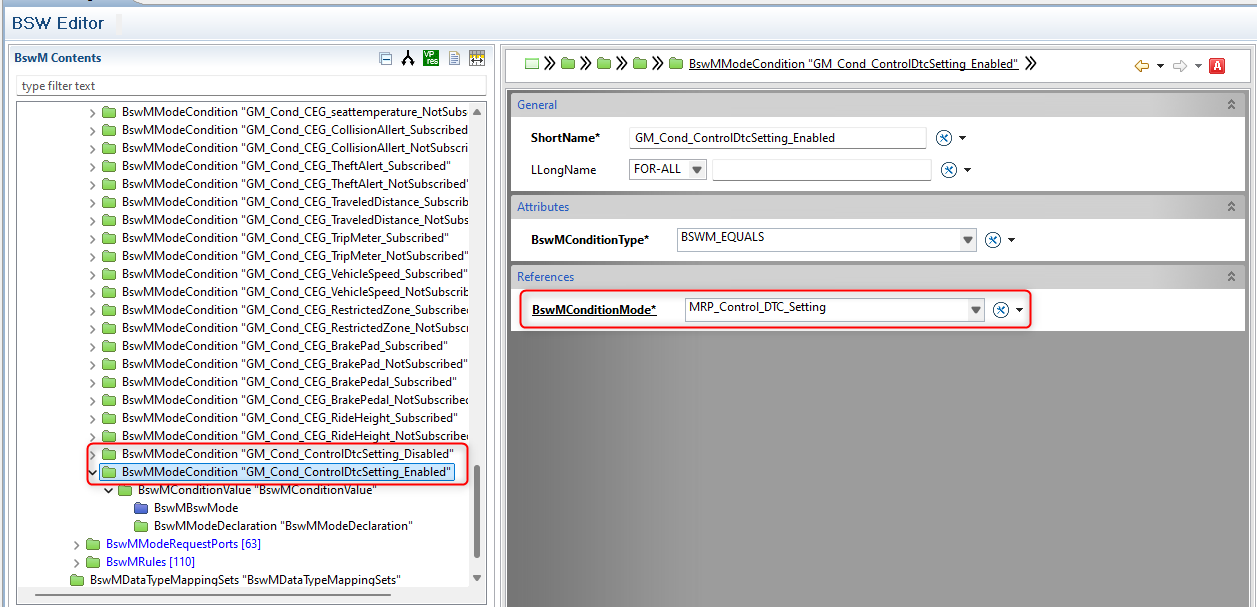
\includegraphics[width=1\textwidth]{images/BswM1.png}
	\caption{Conditions}
	\label{fig:Conditions}
\end{figure} 

\begin{figure}[H]
	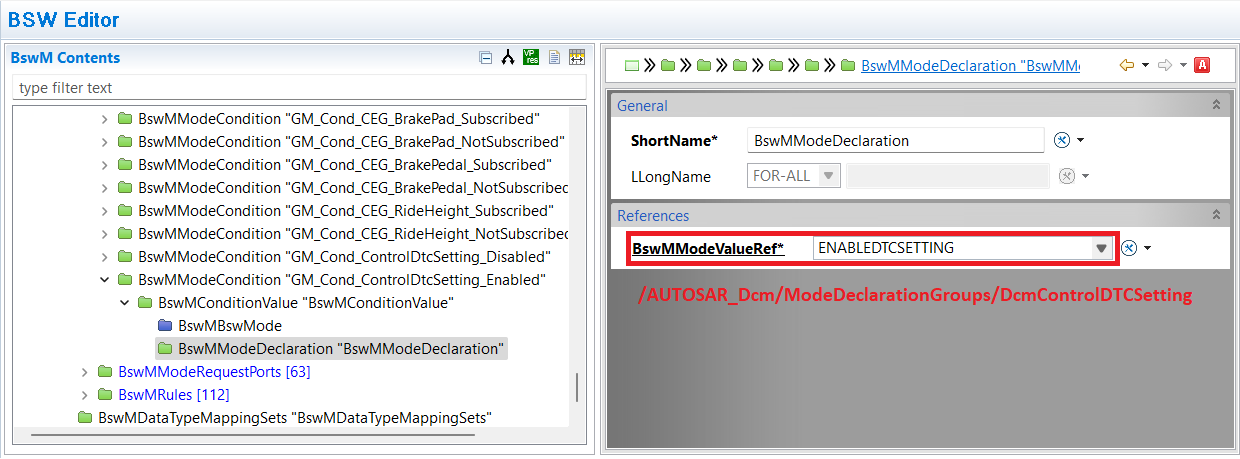
\includegraphics[width=1\textwidth]{images/BswM2.png}
	\caption{Conditions value}
	\label{fig:ConditionsValue}
\end{figure} 

Then, reference them in two different \textit{Logical Expressions}, as in Figure \ref{fig:LogicalExpressions} .

\begin{figure}[H]
	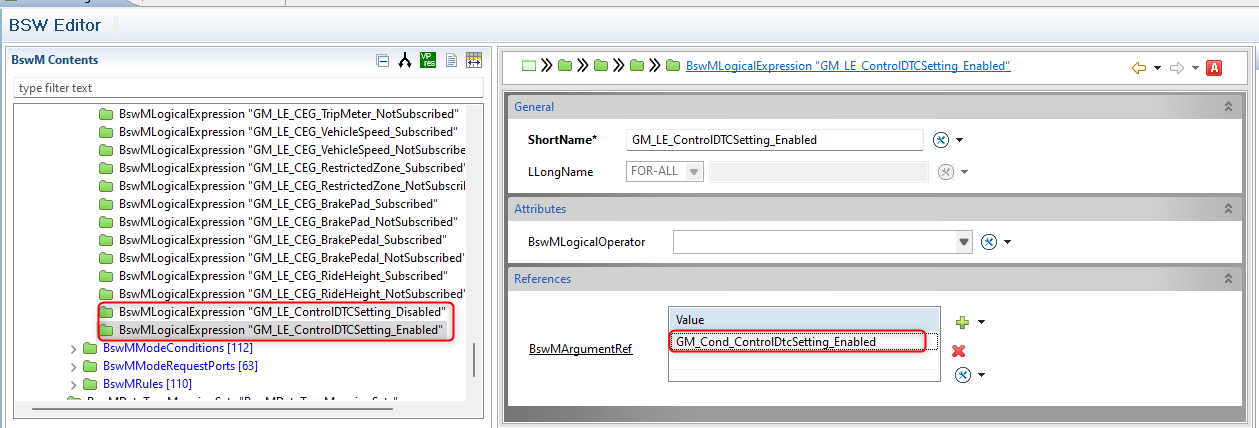
\includegraphics[width=1\textwidth]{images/BswM3.png}
	\caption{Logical Expressions}
	\label{fig:LogicalExpressions}
\end{figure}

Now, we need to create the \textit{BswMSwitchPort} (Figure \ref{fig:BswMRteSwitch} ) that will be used by the actions and rules.
Let's now create two actions for the ENABLED and DISABLED states. For each action, the BswMRteSwitch sub-element should be configured by adding the BswMSwitchPort just created and the corresponding /GM\_SUM/Interfaces/SUM\_ControlDTCSetting/ControlDTCSetting mode (disabled or enabled).

\begin{figure}[H]
	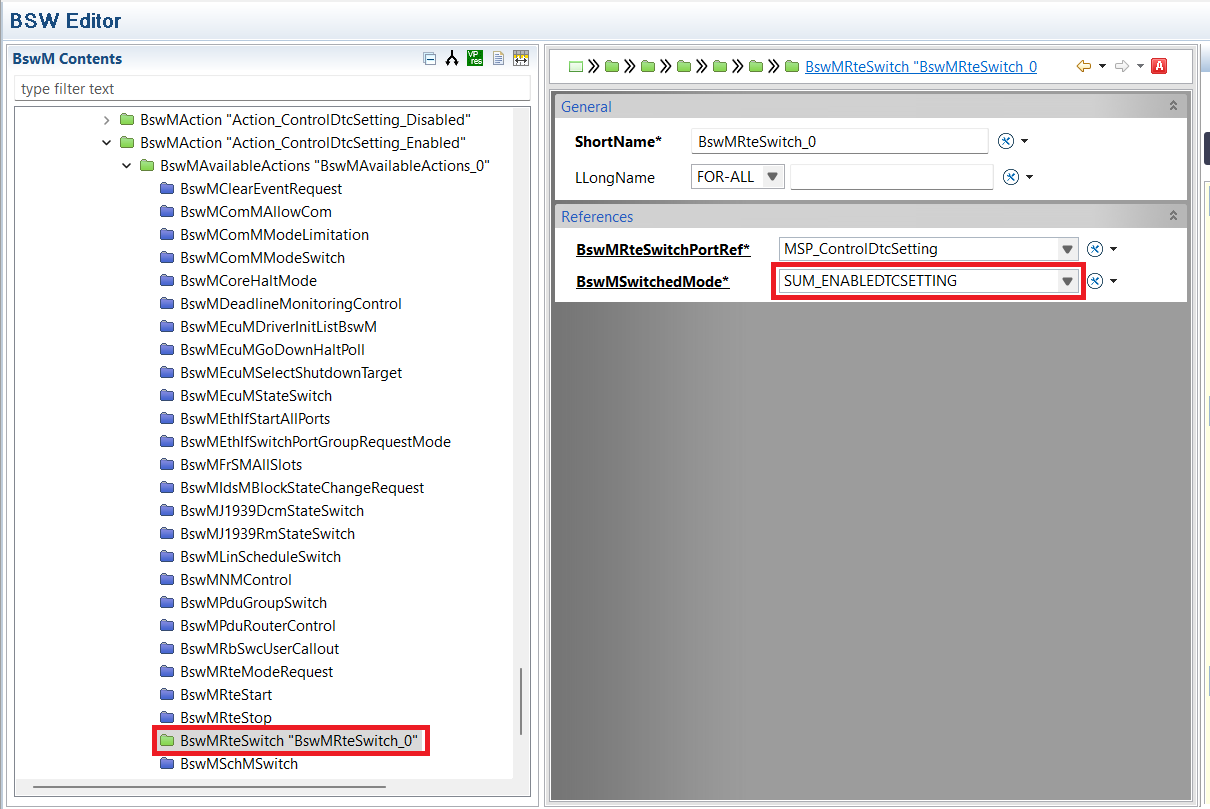
\includegraphics[width=1\textwidth]{images/BswM4.png}
	\caption{BswMRteSwitch}
	\label{fig:BswMRteSwitch}
\end{figure}

Then, we can create two \textit{action lists}  (Figure \ref{fig:actionlist}) to be used later in the rules.
Each of them shall refer one of the two actions created before.

\begin{figure}[H]
	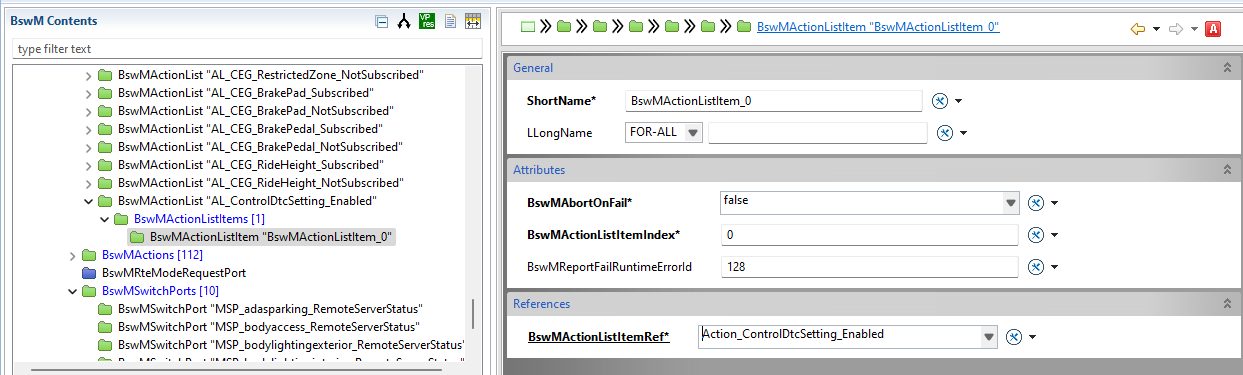
\includegraphics[width=1\textwidth]{images/BswM5.png}
	\caption{Action List}
	\label{fig:actionlist}
\end{figure}

Finally, let's create the \textit{rules}  (Figure \ref{fig:rules}) that will be used to switch the DTC setting control.

\begin{figure}[H]
	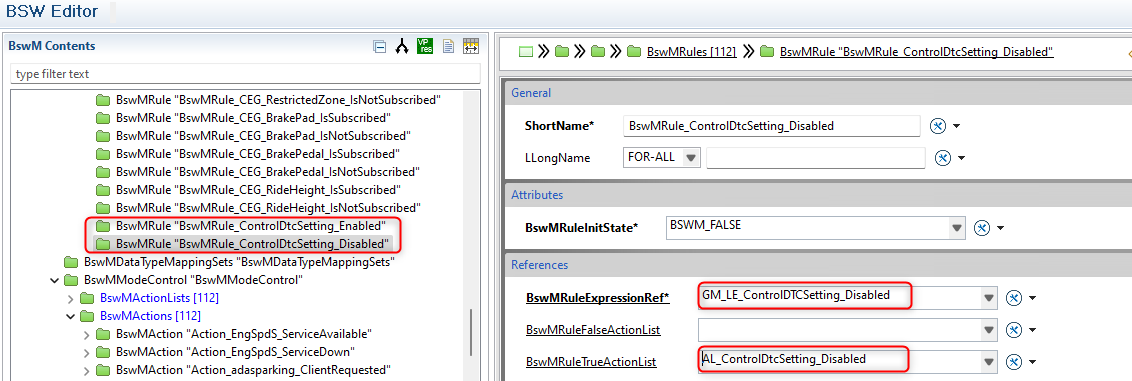
\includegraphics[width=1\textwidth]{images/BswM6.png}
	\caption{Rules}
	\label{fig:rules}
\end{figure}


Update the BswM BswMDataTypeMappingSets to reference the SUM\_ControlDTCSetting interface \newline
data type mapping.

\subsubsection{Module Configuration}
The BswM \textbf{PP\_MSP\_ControlDtcSetting} port shall be configured to use the \newline 
\textbf{/GM\_SUM/Interfaces/SUM\_ControlDTCSetting} interface and connected with the \newline 
\textbf{RP\_DIAG\_BswM\_controlDTCsetting} of the SUM\_DIAG module.

This will trigger two runnables 

\begin{itemize}
	\item \textit{Runnable\_DIAG\_ControlDTCSetting\_Disabled}
	\item \textit{Runnable\_DIAG\_ControlDTCSetting\_Enabled}
\end{itemize}


when the mode changes in the DCM (thanks to the created chain DCM->BswM->SUM\_DIAG).
The runnable, once triggered, will set the InterRunnableVariable for the \textit{ControlDTCSetting} to the corresponding value.
